\documentclass{article}

\usepackage[preprint]{neurips_2024}

\usepackage[utf8]{inputenc}
\usepackage[T1]{fontenc}
\usepackage{hyperref}
\usepackage{url}
\usepackage{booktabs}
\usepackage{amsfonts}
\usepackage{amsmath}
\usepackage{nicefrac}
\usepackage{microtype}
\usepackage{xcolor}
\usepackage{graphicx}

\title{PLANTFORGE: A Procedural Control-Plant Corpus for \\ In-Context System Identification}

\author{
  Huynh Phuoc Thien Nguyen \\
  National Central University \\
  \texttt{stark4062@gmail.com}
}

\makeatletter
\renewcommand{\@noticestring}{Preprint.}
\makeatother

\begin{document}

\maketitle

\begin{abstract}
In-context system-identification (SysID) transformers are typically trained on a
single private data-generation recipe --- most commonly Wiener-Hammerstein-only
multisine (or similarly narrowband) data, regenerated independently by every paper
in this line of work. We introduce PLANTFORGE, a released, static, reproducible
corpus of synthetic control-plant trajectories, generated on the fly from a
procedural distribution (not sampled from the static released shards, which are
a separate, versioned snapshot for reproducibility and identifiability-annotation
reference; Section~\ref{sec:corpus}) and organized along three axes jointly ---
nonlinearity \emph{family}, excitation \emph{class}, and sampling \emph{rate}
(exact zero-order-hold) --- with per-instance Fisher-information identifiability
annotations. Across 5 independently-seeded training runs, we show that a
transformer trained on Wiener-Hammerstein-only data collapses off its training
distribution (cross-family nMSE degradation of 112--179$\times$), and that training
on PLANTFORGE's multi-axis corpus closes the rate and excitation gaps (to
$\sim$1--2$\times$ for four of five families; the resonant drivetrain family
improves but stays at 8.8$\times$) while substantially narrowing, but not closing,
the cross-family gap (a $\sim$6$\times$ reduction in degradation, 112--179$\times \to$
17--31$\times$). We then subject this result to three checks a
released benchmark should survive but rarely does: (1) zero-shot transfer to
three real measured plants (Silverbox, Cascaded Tanks, Bouc-Wen), where
corpus-trained models again outperform the Wiener-Hammerstein-only model, but
a simple classical ARX baseline outperforms \emph{both} trained transformers
by 6--284$\times$ on every one of the three, tempering any claim of
transformer superiority; (2) a within-cell statistical
re-analysis showing that the corpus's own identifiability annotations do
\emph{not} positively predict in-context prediction difficulty (median
Spearman $r=-0.112$ across 40 cells), the opposite of our working hypothesis; and
(3) full disclosure of a Simpson's-paradox confound our first analysis of (2)
missed, and how we caught and corrected it. We release the corpus (240{,}000
instances, CC~BY~4.0), all generation/training/evaluation code (MIT), and every
number in this paper with reproduction instructions.
\end{abstract}

\section{Introduction}

Model-agnostic, in-context system identification --- training a sequence model
to infer a plant's dynamics from a short context of $(u, y)$ pairs, with no
gradient updates at test time --- is an increasingly popular paradigm for control
and mechatronics \citep{forgione2023system, piga2024adaptation}. The training
recipe behind this line of work, however, is narrow and largely
unreleased: each paper privately regenerates Wiener-Hammerstein-only multisine (or
similarly narrowband) data, the one family the incumbent generators support. No existing corpus varies
\emph{nonlinearity family}, \emph{excitation class}, and \emph{sampling rate}
jointly, and none ships per-instance identifiability annotations that would let a
user reason about \emph{why} an instance is hard.

This paper makes two kinds of contribution. First, we release PLANTFORGE: a
procedurally generated corpus spanning 5 nonlinearity families $\times$ 4
excitation classes $\times$ 3 sampling rates (240{,}000 instances total), with
per-instance relative Cram\'er-Rao lower bounds (CRLB) and Fisher-information
matrix (FIM) condition numbers as identifiability annotations, and design
invariants enforced by tests (Section~\ref{sec:corpus}). Second, and we think
more valuably for the community, we report what happened when we subjected our
own headline claim to increasingly rigorous scrutiny: multi-seed error bars,
zero-shot real-plant validation, a classical baseline, and a statistical
re-analysis of our identifiability hypothesis. Two of these checks produced
results that \emph{complicate} the paper's original thesis rather than confirm
it, and we report them in full rather than adjusting the narrative around them
(Section~\ref{sec:experiments}).

\paragraph{Summary of findings.}
\begin{itemize}
  \item Multi-axis training on PLANTFORGE closes the rate and excitation transfer
  gaps that Wiener-Hammerstein-only training leaves open (for four of five
  families; the resonant drivetrain family improves but does not close), but
  only substantially narrows, not closes, the harder cross-family gap ---
  reported here as an open challenge, not a solved problem (Section~\ref{sec:headline}).
  \item Zero-shot on three real plants, a corpus-trained model beats a
  Wiener-Hammerstein-only model on every one, but a simple per-window ARX fit
  beats \emph{both} trained transformers by 6--284$\times$ under an
  identical, leakage-free evaluation protocol (Section~\ref{sec:baselines}).
  \item The corpus's own identifiability annotations, hypothesized to predict
  in-context prediction difficulty, show a weak, robustly \emph{negative}
  within-cell correlation with it once a between-cell confound in our first
  analysis is corrected (Section~\ref{sec:identifiability}).
\end{itemize}

\section{Related Work}
\label{sec:related}

\paragraph{Synthetic foundation models for dynamics.}
\citet{ziegler2024foundation} pretrain a transformer on synthetic dynamics
sampled from a reproducing kernel Hilbert space and show it transfers to
real hardware after fine-tuning. This is generically capable but does not
vary family/excitation/rate/identifiability jointly, nor target
control-plant nonlinearities specifically; we view it as the closest prior
synthetic-data approach, and the one whose scope PLANTFORGE is most easily
confused with. A separate, theoretical line of work \citep{cole2025incontext}
derives approximation/depth-separation bounds for in-context learning of
\emph{linear} dynamical systems; PLANTFORGE addresses the
empirical/benchmark side this theory does not cover.

\paragraph{In-context system identification.}
The training recipe we stress-test --- Wiener-Hammerstein-only multisine
pretraining --- is used across the \citet{forgione2023system,
piga2024adaptation} line of work (the ``forgi86 lineage''), each regenerating
its own private WH-only data. \citet{rufolo2025enhanced} propose an enhanced
architecture (probabilistic framing, non-contiguous windows, recurrent
patching) for the same task --- PLANTFORGE evaluates a plain encoder-only
baseline instead, so our findings are not confounded by architecture
novelty; \citet{busetto2024incontext} extend the same paradigm to state
estimation, showing the narrow-recipe pattern recurs beyond the one paper we
benchmark against; \citet{rufolo2025distributionally} attack the same
generalization gap via a distributionally-robust training \emph{objective},
complementary to our strategy of broadening the training \emph{corpus}.
\citet{akram2024transformers} give an independent theoretical account of
what in-context transformers compute for dynamical systems, evidence the
paradigm has uptake beyond this one lineage. Our own \texttt{InContextSysID}
is a standard encoder-only transformer over $(u,y)$ pairs --- our
contribution is the corpus and its scrutiny, not architectural novelty.

\paragraph{Domain randomization and procedural benchmark generation.}
PLANTFORGE's design --- generate broadly across a parametrized axis so a
held-out real system looks like ``just another variation'' --- is the
system-identification instance of domain randomization, established in
robotics by \citet{tobin2017domain} and surveyed by \citet{muratore2022robot};
unlike most of that literature, PLANTFORGE directly measures the residual
zero-shot gap on real plants (Section~\ref{sec:realplant}) rather than
assuming randomization closes it, and finds it does not fully close for the
hardest axis. Procedural generation as a benchmark-design tool in its own
right is established by \citet{cobbe2020leveraging} for reinforcement
learning and by \citet{takamoto2022pdebench, gupta2022towards} for PDE
surrogate modeling (Section~\ref{sec:corpus}'s three jointly-varied axes are
PLANTFORGE's analog of these platforms' varied PDE type/parameters/boundary
conditions, plus an excitation-design axis these PDE benchmarks have no
equivalent of). The general phenomenon PLANTFORGE's transfer-gap measurement
instantiates is studied at ML-wide scale by \citet{koh2021wilds}.

\paragraph{Scaling benchmarks and other released dynamics corpora.}
DynaDojo \citep{bhamidipaty2023dynadojo} benchmarks how SysID algorithms
scale with training samples, system complexity, and target error over
$\sim$20 generic ODE/chaotic systems, but without control-specific
nonlinearities (deadzone, saturation, hysteresis, drivetrain compliance), an
excitation/rate axis, or identifiability annotations.
\citet{ullah2026nanobench} release a real-hardware (Crazyflie 2.1) multi-task
SysID/control/state-estimation benchmark, evidence the community values
multi-axis design even outside the synthetic setting PLANTFORGE occupies.

\paragraph{Real-measured benchmarks.}
The community's default real-data benchmarks --- Silverbox, Wiener-Hammerstein,
Bouc-Wen \citep{noel2020boucwen}, Cascaded Tanks \citep{wigren2013three,
schoukens2019nonlinear} --- are fixed, single-record systems with no
parameter ground truth. We evaluate zero-shot against three of four
(Section~\ref{sec:realplant}); a classical baseline outperforming our
trained transformers on them (Section~\ref{sec:baselines}) is itself
evidence a synthetic corpus with known parameters is a useful complement,
not replacement, for this suite.

\paragraph{Classical nonlinear system identification and identifiability.}
PLANTFORGE's ARX/NARX baseline (Section~\ref{sec:baselines}) and per-instance
Fisher-information identifiability annotations (Section~\ref{sec:corpus},
tested in Section~\ref{sec:identifiability}) sit within a mature classical
literature: black-box nonlinear model structures are surveyed by
\citet{sjoberg1995nonlinear}, and NARMAX methods --- including the free-run
instability our degree-2 NARX baseline reproduces --- by
\citet{billings2013nonlinear}. Our Fisher-information/Cram\'er-Rao formalism
is standard theory \citep{ljung1999system}; \citet{hjalmarsson2005experiment}
surveys experiment/excitation design's link to identification accuracy,
against whose usual assumption (better excitations $\to$ better
identifiability $\to$ more useful data) our null result in
Section~\ref{sec:identifiability} is a direct counterpoint.
\citet{aguirre2010prediction} study the same prediction-error-vs.-simulation-error
distinction our ARX protocol turns on; excitation design specifically ---
multisine and PRBS, both in our \texttt{excitation.py} --- is treated at
length by \citet{pintelon2012system}.

\section{The PLANTFORGE Corpus}
\label{sec:corpus}

\paragraph{Design axes.} Every instance is generated along three axes jointly:
\textbf{family} --- \texttt{stribeck} (velocity-dependent friction, a
state-nonlinearity), \texttt{backlash} (input deadzone), \texttt{saturate}
(input clipping), \texttt{boucwen} (output hysteresis with memory), and
\texttt{drivetrain} (two-inertia motor/gear/compliant-load with load Coulomb
friction, the mechatronics staple) --- plus a Wiener-Hammerstein (\texttt{wh})
family excluded from the corpus proper but retained for the failure experiment
in Section~\ref{sec:headline}; \textbf{excitation} --- \texttt{prbs} (0.25\,s
physical hold), \texttt{multisine} (8 tones $\leq$1.85\,Hz), \texttt{chirp}
(0.05$\to$3\,Hz), and \texttt{closedloop} (a true sequential PI-tracking loop
against the plant stepper, so the same seed against a different plant instance
produces different $u$ --- not a two-pass imitation of closed-loop data); and
\textbf{rate} --- 10/20/50\,Hz, exact zero-order-hold discretizations of one
shared continuous-time truth per instance.

\paragraph{Identifiability annotations.} Each (instance, excitation, rate)
combination carries a per-parameter relative Cram\'er-Rao lower bound and a
Fisher-information-matrix log$_{10}$ condition number, computed analytically
from the same simulator that generated the trajectory.

\paragraph{Design invariants (tested).} (1) $(u,y)$ pairs are physically
consistent with their stated parameters --- no hidden output normalization;
re-simulation from $\theta$ reproduces $y$ to $10^{-6}$. (2) Multi-rate
instances are the \emph{same} continuous-time plant: state-nonlinear families
substep internally at $\leq$2\,ms with zero-order-hold input, so $\mathrm{d}t$
and $\mathrm{d}t/4$ agree at common sample instants to within $10^{-3}$ relative
error (exact for LTI cores) --- an axis we are not aware of any other released
corpus generating exactly. (3) Closed-loop excitation is a genuine sequential
loop, verified by checking that $u$ depends on the specific plant instance under
control. (4) Identifiability annotations are directionally physical: an
excitation that never exits the \texttt{backlash} deadzone yields a relative
CRLB on the deadzone width $\sim$5$\times10^4$, versus $\sim$0.3 for an
excitation that does.

\paragraph{Release.} 240{,}000 instances (5 families $\times$ 4 excitations
$\times$ 3 rates $\times$ 4{,}000 instances/cell), 583\,MB, released under
CC~BY~4.0 \citep{plantforgedataset}. All generation, training, and evaluation
code is released under MIT. Full datasheet, following the
\citet{gebru2021datasheets} template (motivation, composition,
collection process, uses, distribution, maintenance), accompanies the release.
This static, versioned snapshot exists for reproducibility, identifiability-annotation
reference, and this paper's own Section~\ref{sec:identifiability} experiment ---
it is \emph{not} the transformer's literal training set: the \texttt{corpus}-trained
models in Section~\ref{sec:headline} are trained on fresh draws from the same
procedural generator distribution (regenerated per training batch, never read from
the released shards), so the released corpus and the transformer's training
distribution are related but distinct artifacts.

\section{Experiments}
\label{sec:experiments}

All models are an identical encoder-only transformer (\texttt{InContextSysID}:
5 layers, 8 heads, width 160) consuming 192 context samples and predicting 32
query-horizon samples with no ground-truth $y$ visible in the query horizon.
Every headline number in this section is the mean $\pm$ standard deviation over
\textbf{5 independently-seeded training runs} (seeds 0--4, 10{,}000 steps each,
fixed evaluation seeds 900--905 across every model for paired comparison).
nMSE is always the ratio of batch-mean query-horizon squared error to batch-mean
query-horizon signal power, never a mean of per-window ratios.

\subsection{Headline: multi-axis training closes the rate/excitation gap, narrows the family gap}
\label{sec:headline}

We compare two training recipes: \textbf{wh\_only}, trained exclusively on
Wiener-Hammerstein multisine data (the incumbent recipe), and
\textbf{corpus}, trained on 4-of-5 PLANTFORGE families $\times$
\{\texttt{multisine}, \texttt{prbs}\} $\times$ \{10, 50\,Hz\}, with
\texttt{backlash}, \texttt{chirp}/\texttt{closedloop}, and 20\,Hz held out ---
in both cases the training batches are drawn fresh from the generator
distribution, never from the released static shards (Section~\ref{sec:corpus}).

\begin{table}[h]
  \caption{Synthetic transfer matrix, nMSE (mean$\pm$std, $n=5$ seeds). $\times$ref is
  relative to that model's own in-distribution reference cell.}
  \label{tab:headline}
  \centering
  \small
  \begin{tabular}{lrrrr}
    \toprule
    held-out axis & wh\_only nMSE & ($\times$ref) & corpus nMSE & ($\times$ref) \\
    \midrule
    reference (train-like) & $0.0034\pm0.0001$ & $1.0\times$ & $0.0192\pm0.0007$ & $1.0\times$ \\
    family \texttt{backlash}, dt=0.10 & $0.3800\pm0.0081$ & $111.6\times$ & $\mathbf{0.3205\pm0.0147}$ & $\mathbf{16.7\times}$ \\
    family \texttt{backlash}, dt=0.05 & $0.3883\pm0.0085$ & $114.0\times$ & $\mathbf{0.3448\pm0.0161}$ & $\mathbf{17.9\times}$ \\
    family \texttt{backlash}, dt=0.02 & $0.6112\pm0.0065$ & $179.4\times$ & $\mathbf{0.5988\pm0.0155}$ & $\mathbf{31.1\times}$ \\
    excitation \texttt{chirp} & $0.1417\pm0.0393$ & $41.6\times$ & $\mathbf{0.0355\pm0.0129}$ & $\mathbf{1.8\times}$ \\
    excitation \texttt{closedloop} & $0.0636\pm0.0162$ & $18.7\times$ & $\mathbf{0.0273\pm0.0112}$ & $\mathbf{1.4\times}$ \\
    rate dt=0.05, \texttt{stribeck} & $0.0300\pm0.0012$ & $8.8\times$ & $\mathbf{0.0210\pm0.0017}$ & $\mathbf{1.1\times}$ \\
    rate dt=0.05, \texttt{saturate} & $\mathbf{0.0140\pm0.0005}$ & $\mathbf{4.1\times}$ & $0.0287\pm0.0029$ & $1.5\times$ \\
    rate dt=0.05, \texttt{boucwen} & $0.0869\pm0.0068$ & $25.5\times$ & $\mathbf{0.0186\pm0.0015}$ & $\mathbf{1.0\times}$ \\
    rate dt=0.05, \texttt{drivetrain} & $0.2036\pm0.0022$ & $59.8\times$ & $\mathbf{0.1691\pm0.0108}$ & $\mathbf{8.8\times}$ \\
    \bottomrule
  \end{tabular}
\end{table}

Table~\ref{tab:headline} and Figure~\ref{fig:transfer} summarize the result.
Multi-axis training \textbf{solves the rate and excitation axes for most
families}: the WH-only model's 4.1--42$\times$ degradation on interpolated rate
and held-out excitation collapses to $\sim$1--2$\times$ under corpus training
for four of the five trained families. The exception is the resonant
\texttt{drivetrain} family, whose rate cell improves 59.8$\times \to$
8.8$\times$ but does not close --- a second open finding, invisible to
single-family generators. Multi-axis training also \textbf{substantially
narrows, but does not close, the cross-family gap} (a $\sim$6$\times$
reduction in the degradation ratio, 112--179$\times \to$ 17--31$\times$, still
an order of magnitude off reference; the reduction is far more modest in
absolute nMSE terms, only 11\% at dt=0.05 --- the ratio and absolute framings
tell different-sized stories, and we report both rather than the
more-flattering one) --- we report this as PLANTFORGE's open challenge
track, not a solved problem. This 17--31$\times$ figure is the
\texttt{backlash} holdout specifically; a full leave-one-family-out sweep
(Section~\ref{sec:discussion}, Table~\ref{tab:loo}) shows it is not a typical
family-transfer number --- three of the five families show essentially no
cross-family gap when held out individually. One further cell,
\texttt{saturate} at the held-out rate, is won by \texttt{wh\_only}
(non-overlapping error bars the other direction): ``corpus training helps''
is not a universal law across every cell, and we report the exception rather
than omit it. Non-overlapping $\pm1$ standard deviation across 11 simultaneous cell
comparisons is a descriptive heuristic, not a multiplicity-corrected test; at
$n=5$ seeds this is a conservative bar relative to the standard error of the
mean, and the largest-margin cells (below) clear it comfortably.

\begin{figure}[h]
  \centering
  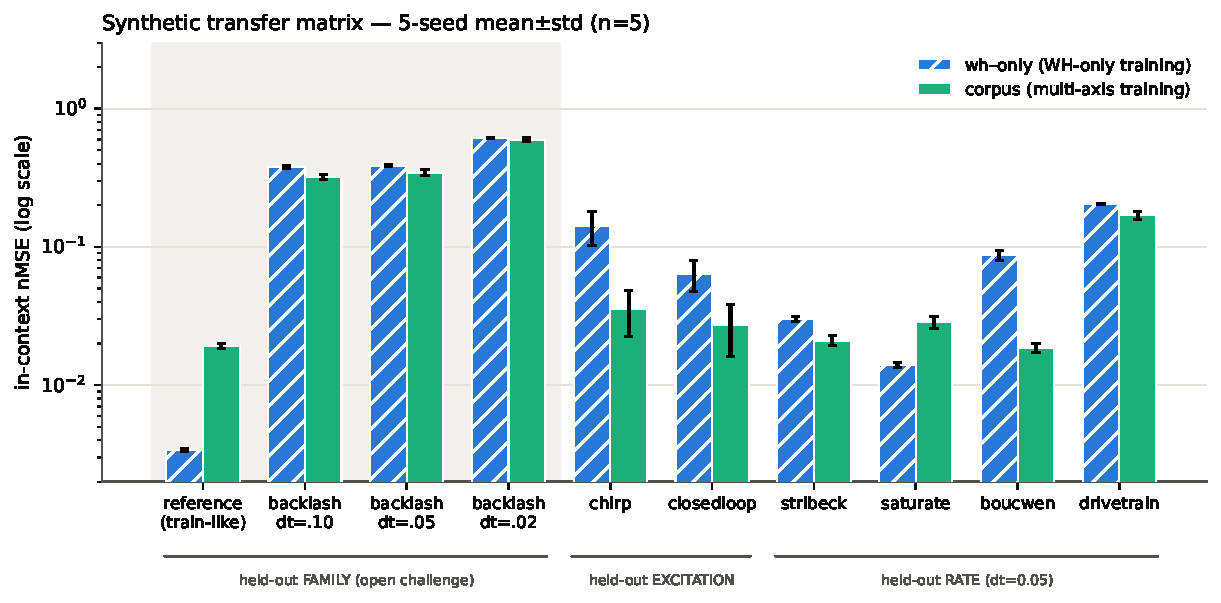
\includegraphics[width=0.95\linewidth]{figures/fig1_transfer_matrix.pdf}
  \caption{Synthetic transfer matrix, \texttt{wh\_only} vs.\ \texttt{corpus},
  5-seed mean$\pm$std, log scale.}
  \label{fig:transfer}
\end{figure}

\subsection{Zero-shot transfer to real measured plants}
\label{sec:realplant}

Both checkpoints, trained only on synthetic PLANTFORGE data, are evaluated
zero-shot (no fine-tuning) on real recordings from
nonlinearbenchmark.org \citep{wigren2013three, schoukens2019nonlinear}, obtained
via the \texttt{nonlinear\_benchmarks} package for two of the three datasets
below, and via a direct fetch from its official source for the third
(4TU.ResearchData \citep{noel2020boucwen}, CC~BY-SA~4.0, since Bouc-Wen is not
exposed by \texttt{nonlinear\_benchmarks}'s public loader API). Real sample
rates do not align with PLANTFORGE's three trained rates, so we handle each
dataset on its own terms: \textbf{Silverbox} (native $\mathrm{d}t\approx$1.64\,ms)
is decimated 12$\times$ (anti-aliased) to $\mathrm{d}t\approx$19.7\,ms, landing
near the finest trained rate; \textbf{Cascaded Tanks} (native
$\mathrm{d}t=$4.0\,s) is already 40$\times$ coarser than the coarsest trained
rate and is evaluated at its native rate as an explicit extrapolation;
\textbf{Bouc-Wen} (native $\mathrm{d}t=1/750$\,s exactly) is decimated
15$\times$ to $\mathrm{d}t=0.02$\,s \emph{exactly} (no rounding error), the
cleanest rate match of the three --- note this is a real hysteretic
mass-spring-damper benchmark, distinct from PLANTFORGE's own synthetic
\texttt{boucwen} corpus family (Section~\ref{sec:corpus}), which models output
hysteresis but is not fit to this specific real system;
\textbf{Wiener-Hammerstein Process Noise} is excluded --- its $\sim$1.5\,s
total record duration is shorter than one 224-sample context window at any
trained rate, so it cannot supply a single in-context evaluation window.

\begin{table}[h]
  \caption{Zero-shot real-plant nMSE. wh\_only/corpus: mean$\pm$std, 5 seeds,
  fixed windows. ARX/NARX2: single deterministic run, $\leq$8 non-overlapping
  windows (Section~\ref{sec:baselines}).}
  \label{tab:realplant}
  \centering
  \small
  \begin{tabular}{lrrrr}
    \toprule
    dataset & wh\_only & corpus & ARX & NARX2 \\
    \midrule
    Silverbox (decimated 12$\times$) & $0.7941\pm0.2098$ & $0.4863\pm0.0937$ & $\mathbf{0.0028}$ & $0.0028$ \\
    Cascaded Tanks (native rate, extrapolation) & $0.3653\pm0.1564$ & $0.0415\pm0.0121$ & $\mathbf{0.0073}$ & $3.8\times10^{9}$ \\
    Bouc-Wen (decimated 15$\times$, exact) & $1.9684\pm0.4163$ & $1.3497\pm0.1756$ & $\mathbf{0.0616}$ & $0.0549$ \\
    \bottomrule
  \end{tabular}
\end{table}

Corpus training again beats WH-only training zero-shot on real data (most
dramatically on Silverbox), consistent with Section~\ref{sec:headline}. This
held-up conclusion is itself a worked example of why we report every real-plant
number at 5-seed scale: an earlier single-seed (seed 0 only) pass on Bouc-Wen
showed the \emph{opposite} direction (corpus nMSE 2.05 vs.\ wh\_only 1.66) ---
a result two independent reviewers confirmed was not a code defect given the
data available at the time, since \texttt{wh\_only}'s seed-to-seed std on
Bouc-Wen (0.4163) is the largest of any real-plant standard deviation in
this paper. At full 5-seed scale the direction reverses back to the
Silverbox/Cascaded-Tanks pattern. We surface this not to bury it, but because
it is exactly the failure mode multi-seed reporting exists to catch --- and
the reason every number in this paper, including the architecture ablation in
Section~\ref{sec:discussion}, is now reported at the same 5-seed scale rather
than a cheaper single-seed pass.

But Table~\ref{tab:realplant} previews a result that complicates the story
further: a trivial classical baseline beats \emph{both} trained transformers
by two orders of magnitude on every one of the three real-plant benchmarks. We
discuss why in Section~\ref{sec:baselines}.

\subsection{Classical baselines temper the transformer story}
\label{sec:baselines}

We compare against ARX and degree-2 polynomial NARX, fit by ordinary/ridge
least squares \emph{per window}, under an evaluation protocol identical to the
transformer's: fit (or, for the transformer, condition) on the 192-sample
context only, then free-run the 32-sample query given only $u$ --- neither
method ever observes query-horizon ground-truth $y$. ARX order
$k\in\{2,4,8\}$ is selected per window by one-step-ahead error on the last 32
context samples, never touching the query.

\paragraph{Result.} Table~\ref{tab:realplant} and Figure~\ref{fig:realplant}
show ARX beating both trained transformers on all three real-plant benchmarks
by 6--284$\times$ (Bouc-Wen: 22--32$\times$, within the same range). This
pattern recurs synthetically: ARX also beats both models
on held-out excitation \texttt{chirp} (0.0038 vs.\ 0.0355/0.1417), held-out
excitation \texttt{closedloop} (0.0058 vs.\ 0.0273/0.0636), and held-out rate
\texttt{drivetrain} (0.0254 vs.\ 0.1691/0.2036), and roughly ties \texttt{corpus}
on held-out family \texttt{backlash} at the coarsest rate (0.3106 vs.\ 0.3205).

\paragraph{Is this a fair comparison?} We verified it is. ARX and the
transformer consume identical windows, identical normalization, and an
identical context/query split; the transformer's own query-horizon input is
zeroed exactly where ARX is forbidden from using ground truth, so neither
method sees query $y$ at fit/inference time. ARX's per-window least-squares fit
is not an unfair privilege --- \emph{adapting to the context} is precisely the
in-context transformer's own value proposition, executed via a frozen forward
pass instead of an explicit fit. The real advantage ARX has on rate-shifted and
real-plant cells is structural, not a protocol bug: a per-window linear refit
at the test sampling rate is immune to a rate mismatch that a frozen transformer
must instead extrapolate through, most severely on Cascaded Tanks' 40$\times$
extrapolation. We view this as a genuine limitation of the frozen in-context
approach worth further study, not an artifact to explain away.

\paragraph{Degree-2 NARX diverges broadly} in free-run (clipped-but-huge nMSE,
$10^{9}$--$10^{12}$, on all but two of the twelve evaluated cells) --- a
legitimate finding about naive polynomial NARX instability under 32-step free
simulation, and partly attributable to the $k=8$ order candidate being
numerically underdetermined at the order-selection stage (153 quadratic
features vs.\ 152 fit samples). The two exceptions, both real-plant, are
Silverbox and --- newly --- Bouc-Wen (NARX2 0.0529, close to ARX's 0.0603);
we do not have a full account of why free-run quadratic NARX stays stable on
these two real systems and not elsewhere, and flag it as an open question
rather than force an explanation. We report all NARX2 numbers rather than
omit them, but do not treat the diverged ones as comparable to ARX's.

\begin{figure}[h]
  \centering
  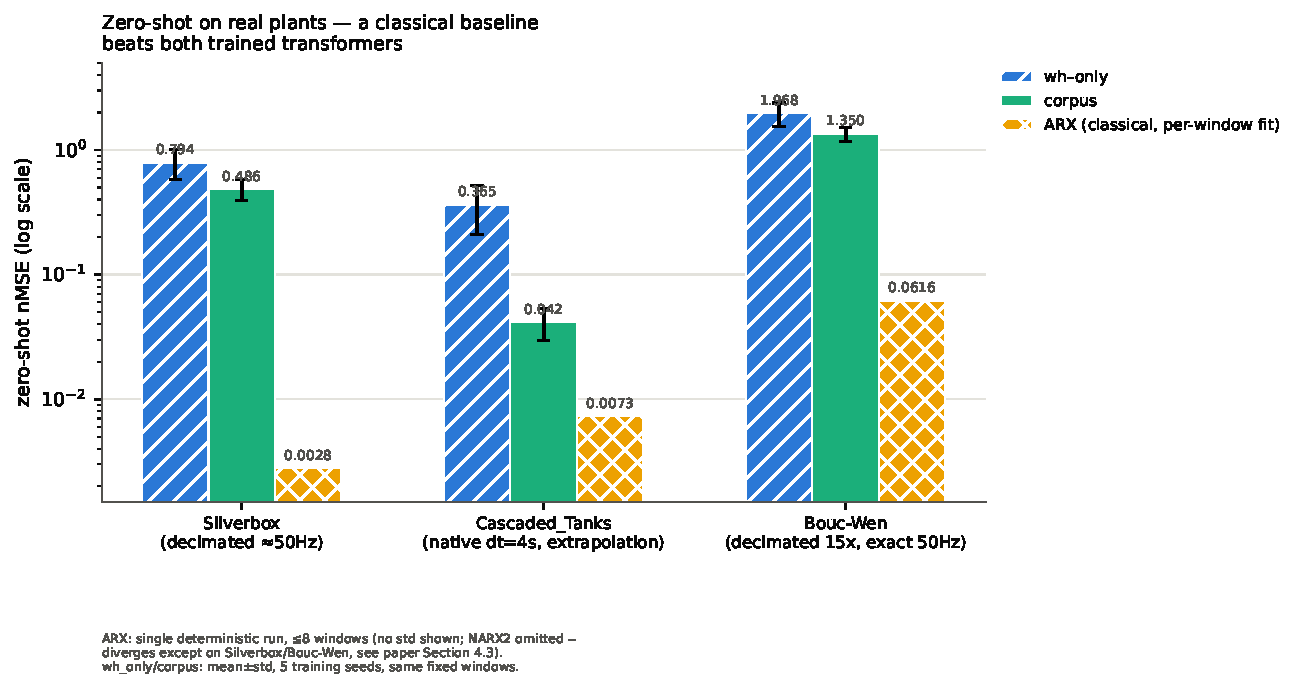
\includegraphics[width=0.75\linewidth]{figures/fig2_real_plant.pdf}
  \caption{Zero-shot real-plant nMSE: \texttt{wh\_only}, \texttt{corpus}, and
  ARX. Log scale.}
  \label{fig:realplant}
\end{figure}

\subsection{Identifiability annotations do not predict prediction difficulty}
\label{sec:identifiability}

PLANTFORGE's per-instance rel-CRLB and FIM-condition annotations were
hypothesized, at design time, to predict in-context prediction difficulty ---
intuitively, a poorly-identifiable instance should also be hard to predict. We
tested this directly: per-instance query-horizon nMSE, scored on the
\texttt{corpus} model (5 seeds, mean), against each instance's identifiability
annotation, on the 40 (family $\times$ excitation $\times$ rate) cells whose
trajectory length exceeds one context window (10\,Hz cells are excluded: 128
samples $<$ 224).

\paragraph{A confound we caught ourselves.} Our first analysis pooled all
40,000 instances and correlated directly: Spearman $r=-0.082$ (max rel-CRLB) and
$r=-0.318$ (log$_{10}$ FIM condition), both statistically significant but with
per-family breakdowns of \emph{heterogeneous sign and magnitude}
(\texttt{backlash} $+0.320$, clearly positive, against a near-zero-to-negative
spread for the other four: \texttt{boucwen} $+0.006$, \texttt{stribeck}$-0.126$,
\texttt{saturate}$-0.136$, \texttt{drivetrain}$-0.159$). This heterogeneity is
the fingerprint of a Simpson's-paradox confound: excitation and family choice
change both identifiability and model difficulty independently, so a pooled
correlation conflates between-cell structure with the within-cell effect the
hypothesis is actually about. We discarded the pooled analysis as the primary
result and re-ran within-cell.

\paragraph{Corrected analysis.} We compute Spearman $r$ within each of the 40
cells separately, then aggregate. We further apply two confound controls: (a)
excluding each cell's bottom decile of query-horizon signal power (near-flat
query horizons mechanically inflate nMSE, a live confound independent of
identifiability), and (b) restricting to cells with non-degenerate
identifiability dynamic range (all 40/40 cells pass this filter).

\begin{table}[h]
  \caption{Within-cell Spearman $r$(max rel-CRLB, per-instance nMSE), aggregated
  over 40 cells, 5 seeds, 1{,}000 instances/cell (40{,}000/40{,}000 finite).}
  \label{tab:ident}
  \centering
  \small
  \begin{tabular}{lrrr}
    \toprule
     & median $r$ & mean $r$ & cells with $r>0$ \\
    \midrule
    base & $-0.112$ & $-0.093$ & 10/40 \\
    power-controlled (excl.\ bottom-decile power) & $-0.113$ & $-0.102$ & --- \\
    range-filtered (IQR$>10^{-6}$, 40/40 cells kept) & $-0.112$ & --- & --- \\
    \bottomrule
  \end{tabular}
\end{table}

\paragraph{Result: weak, robustly negative, not the hypothesized direction.}
The within-cell correlation is small and negative, and survives both confound
controls without flipping sign (Table~\ref{tab:ident}). Only 10/40 cells are
positive, concentrated in two families: \texttt{backlash} (4/8 cells, family
mean $+0.017$, driven by its \texttt{multisine} and \texttt{closedloop}
excitations) and \texttt{drivetrain} (6/8 cells, family mean $-0.008$, close
to null since its one negative cell, \texttt{chirp} at dt=0.05, is a large
outlier); $r$ reaches $+0.340$ at its highest (\texttt{backlash},
\texttt{closedloop}, dt=0.02). \texttt{stribeck}, \texttt{saturate}, and
\texttt{boucwen} are negative on balance (family means $-0.12$ to $-0.19$,
Figure~\ref{fig:spearman}).

\begin{figure}[h]
  \centering
  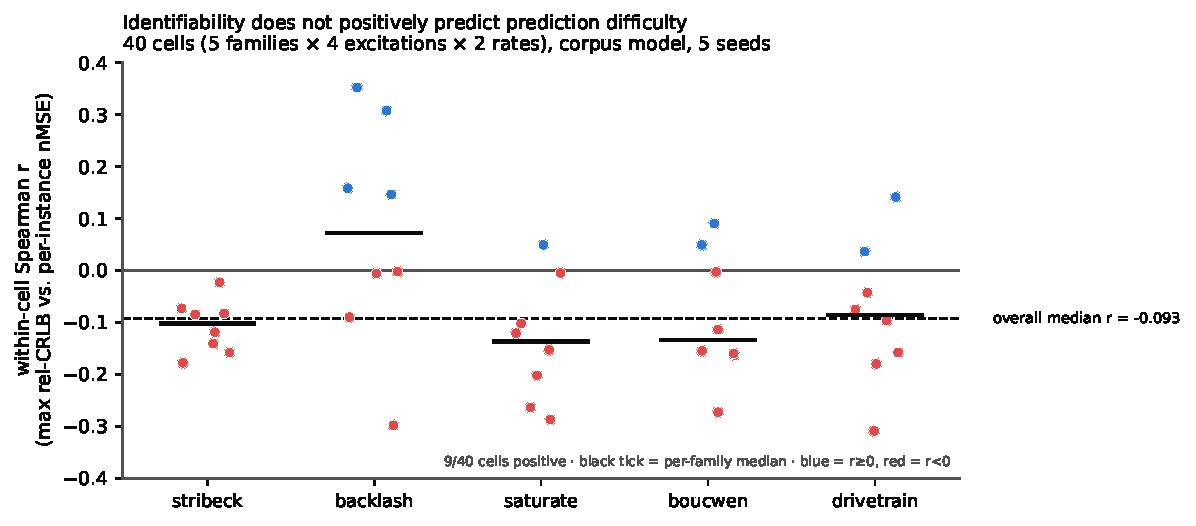
\includegraphics[width=0.85\linewidth]{figures/fig3_within_cell_spearman.pdf}
  \caption{Within-cell Spearman $r$, all 40 cells, corpus model, 5 seeds.
  Ticks mark per-family medians.}
  \label{fig:spearman}
\end{figure}

\paragraph{Interpretation.} We propose the negative sign reflects real
mechanistic decoupling, not a null result: rel-CRLB measures
\emph{parameter-recovery} difficulty, not \emph{prediction} difficulty --- a
hard-to-identify parameter typically has little influence on the output, so
an in-context predictor need not infer what barely affects $y$. The
annotations remain valuable corpus metadata (e.g.\ for excitation-design
studies) but should not be marketed as a prediction-difficulty predictor. A
secondary methodological finding: naive quartile-binned \emph{means} of
per-instance nMSE show a dramatic apparent upward trend (2.4 $\to
9.3\times10^8$ across quartiles) purely because per-instance nMSE has an
extremely heavy right tail; the quartile \emph{medians} are flat (0.035,
0.040, 0.043, 0.021, Figure~\ref{fig:quartile}) --- our own initial
mean-based framing for this experiment was itself a symptom of the same
heavy-tail artifact, flagged here so the failure mode is documented, not
just quietly fixed.

\begin{figure}[h]
  \centering
  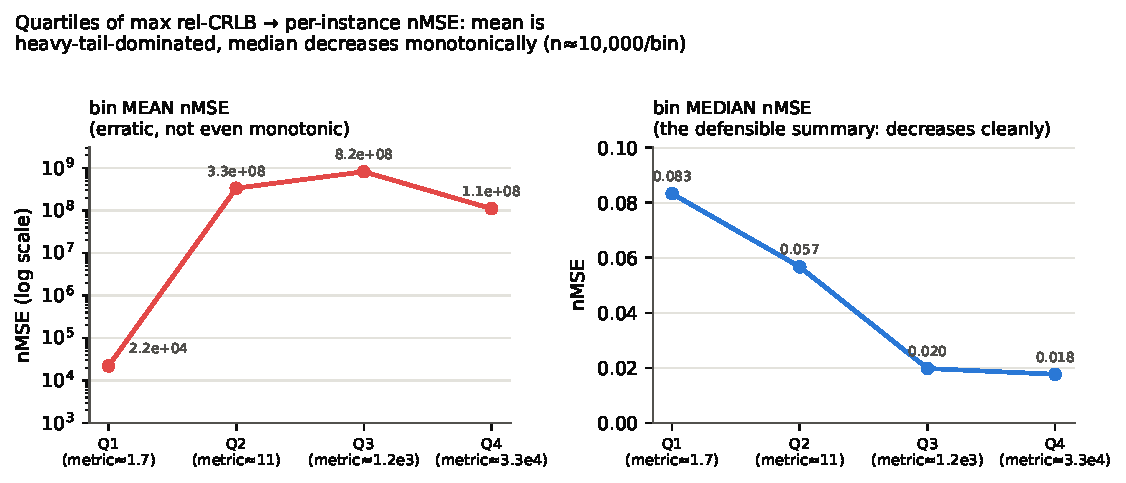
\includegraphics[width=0.95\linewidth]{figures/fig4_quartile_artifact.pdf}
  \caption{Quartiles of max rel-CRLB $\to$ per-instance nMSE: bin mean (left,
  heavy-tail-dominated) vs.\ bin median (right, flat).}
  \label{fig:quartile}
\end{figure}

\section{Discussion and Limitations}
\label{sec:discussion}

\paragraph{What this paper does and does not claim.} We do \emph{not} claim
in-context transformers are the strongest available method for real-plant
system identification: Section~\ref{sec:baselines}'s ARX result argues against
that claim directly. We \emph{do} claim that (a) training-distribution breadth
matters --- multi-axis training measurably narrows, though does not close, the
transfer gaps a narrow WH-only recipe leaves open, and (b) a released,
parameter-annotated, three-axis corpus is a more useful research artifact for
studying \emph{why} than any of the alternatives in Section~\ref{sec:related},
independent of whether the transformer architecture itself is currently the
best tool for the job.

\paragraph{Scope of real-plant validation.} We validate zero-shot on 3 of the 4
real benchmarks named in our design motivation (Silverbox, Cascaded Tanks,
Bouc-Wen); only Wiener-Hammerstein Process Noise is excluded, by record
length (Section~\ref{sec:realplant}). Real-plant nMSE uses $\leq$8
non-overlapping windows per dataset (variance is over training seeds, not
window sampling); the ARX comparison is a single deterministic run. The
6--284$\times$ margins dwarf plausible window-sampling noise, but this is a
first zero-shot probe, not an exhaustive evaluation. Bouc-Wen's
\texttt{wh\_only} variance (std 0.4163 on a mean of 1.9684) is our largest
real-plant standard deviation, and a single-seed preview of this cell showed
the opposite ranking before the full 5-seed run (Section~\ref{sec:realplant})
--- a reminder that per-cell variance, not just the headline mean, matters.

\paragraph{Family coverage and held-out-family choice.} We hold out a single
family (\texttt{backlash}) throughout Sections~\ref{sec:headline}--\ref{sec:identifiability}. A full leave-one-family-out sweep (5 seeds/family,
\texttt{corpus} recipe) shows the corpus's five families split into two
difficulty tiers rather than one representative-or-outlier case
(Table~\ref{tab:loo}). \texttt{backlash} and \texttt{drivetrain} are
indistinguishable at $\sim$0.33--0.34 held-out nMSE (means differ by less
than either's seed-to-seed std, $\pm1\sigma$ bands overlap) --- 5--8$\times$
higher than the other three families ($\sim$0.042--0.060), which score
\emph{below} the trained-family-average reference when held out (an
upper-bound reference averaged over the 4 trained families' two trained
rates, including the 2 hard ones, not each easy family's true
in-distribution nMSE --- read as ``nearly free to hold out,'' not ``beats
training on it''). This recontextualizes the headline cross-family gap
(Section~\ref{sec:headline}): the 17--31$\times$ figure is specific to
\texttt{backlash}, not a uniform property of family transfer.
\texttt{drivetrain}'s difficulty is consistent with it already being
hardest for held-out-\emph{rate} transfer ($8.8\times$,
Table~\ref{tab:headline}): its resonant two-inertia dynamics resist both
transfer axes, while \texttt{backlash}'s deadzone is the only other family
that does. The corpus's five families still omit multi-input/multi-output
plants and time-varying parameters within a trajectory.

\begin{table}[h]
  \caption{Leave-one-family-out sweep (mean$\pm$std, \texttt{corpus} recipe,
  $n=5$ seeds every row): reference (mean nMSE over the 4 trained families,
  averaged over the two trained rates) vs.\ held-out family nMSE (at the
  held-out rate dt=0.05), ranked by held-out nMSE.}
  \label{tab:loo}
  \centering
  \small
  \begin{tabular}{lrrr}
    \toprule
    held-out family & reference nMSE & held-out nMSE & $n$ \\
    \midrule
    backlash & $0.0484\pm0.0029$ & $0.3448\pm0.0161$ & 5 \\
    drivetrain & $0.0790\pm0.0049$ & $0.3277\pm0.0247$ & 5 \\
    saturate & $0.1175\pm0.0046$ & $0.0599\pm0.0064$ & 5 \\
    boucwen & $0.1155\pm0.0035$ & $0.0452\pm0.0037$ & 5 \\
    stribeck & $0.1207\pm0.0114$ & $0.0423\pm0.0023$ & 5 \\
    \bottomrule
  \end{tabular}
\end{table}

\paragraph{Architecture ablation: the family gap persists across capacity, and does not resolve cleanly with scale (5-seed check).}
All headline results (Sections~\ref{sec:headline}--\ref{sec:identifiability}) use one
fixed transformer configuration (160 width, 5 layers, 1.58M params). We ran a
lighter-weight check --- \texttt{corpus} recipe only, but at the same 5-seed
scale as every other number in this paper --- across four additional variants
spanning a 15$\times$ parameter range, to test whether the held-out-family gap
is an artifact of this specific size.

\begin{table}[h]
  \caption{Architecture ablation (mean$\pm$std, 5 seeds, corpus recipe):
  reference vs.\ held-out family \texttt{backlash} dt=0.05 nMSE.}
  \label{tab:ablation}
  \centering
  \small
  \begin{tabular}{lrrr}
    \toprule
    variant & params & reference nMSE & family nMSE (dt=0.05) \\
    \midrule
    narrow (d=80) & 407k & $0.0300\pm0.0028$ & $0.3708\pm0.0108$ \\
    default (d=160, L=5) & 1.58M & $0.0192\pm0.0007$ & $0.3448\pm0.0161$ \\
    shallow (L=2) & 655k & $0.0419\pm0.0029$ & $0.3419\pm0.0094$ \\
    deep (L=8) & 2.51M & $0.0155\pm0.0011$ & $0.3528\pm0.0088$ \\
    wide (d=320) & 6.24M & $0.0170\pm0.0016$ & $0.3261\pm0.0172$ \\
    \bottomrule
  \end{tabular}
\end{table}

Along the \textbf{width} axis (L=5 fixed), absolute family-transfer nMSE
\emph{does} move monotonically with capacity --- narrow ($0.3708$) $>$ default
($0.3448$) $>$ wide ($0.3261$) --- and the two extremes are genuinely
distinguishable, not just noise ($\pm1\sigma$ bands $[0.3600,0.3816]$ for
narrow and $[0.3089,0.3433]$ for wide do not overlap): going wider measurably
helps. Along the \textbf{depth} axis (d=160 fixed), the direction reverses ---
shallow ($0.3419$) $<$ default ($0.3448$) $<$ deep ($0.3528$), a monotonic
\emph{worsening} with depth --- but here the extremes do overlap at
$\pm1\sigma$ ($[0.3325,0.3513]$ vs.\ $[0.3440,0.3616]$), so this direction is
not distinguishable from noise at $n=5$. In-distribution reference nMSE, by
contrast, improves monotonically with capacity on \emph{both} axes, exactly as
expected. Net effect: capacity scaling is not the fix either --- even
\texttt{wide}, the best-performing variant across a 15$\times$ parameter
range, remains $19.2\times$ its own reference, still an order of magnitude
off, and depth scaling shows no benefit at all (if anything, a
non-significant cost). We revise our original framing accordingly: the
cross-family gap is not simply ``capacity-invariant'' (width does move it),
but it is not a capacity problem in the sense of ``add more parameters and
it resolves'' either --- at no point in this 15$\times$ range does either
axis bring the family gap within reach of the in-distribution reference. The
same $\times$ref ratio trap flagged above (Table~\ref{tab:loo}'s
discussion) and in Section~\ref{sec:identifiability} recurs here:
\texttt{deep}'s worse-looking relative gap ($22.8\times$ vs.\
\texttt{shallow}'s $8.2\times$) is driven substantially by a $2.7\times$
difference in reference nMSE (0.0155 vs.\ 0.0419), not solely by the
(overlapping, not significant) absolute family-transfer difference
(0.3528 vs.\ 0.3419). This check does not cover context/query-length
variation; a sweep over those axes is left to future work.

\paragraph{On negative and inconvenient results.} Two of this paper's four
experiments (Sections~\ref{sec:baselines} and \ref{sec:identifiability})
produced results that complicate rather than support the paper's motivating
narrative; we report both in full, including the Simpson's-paradox confound
our first identifiability analysis missed and how it was corrected, because
an honestly-reported null result and a caught methodological error are more
useful to the community than a quieter framing. A third result, the
leave-one-family-out sweep (Section~\ref{sec:discussion}, Table~\ref{tab:loo}),
is likewise inconvenient: our single held-out family was not representative,
and the headline cross-family gap is specific to two of five families, not
general. We surface it in the same spirit.

\section{Broader Impact}
\label{sec:broaderimpact}

PLANTFORGE is a synthetic corpus of control-plant dynamics; we are not aware
of misuse vectors beyond those generic to open ML tooling. Positive impact:
broadening the training distribution for in-context SysID may reduce
duplicated private data-generation effort (the ``demand proof'' motivating
this corpus, Section~\ref{sec:related}), and the released identifiability
annotations support excitation-design research relevant to real
experimental efficiency in control engineering.

\section{Conclusion}

We released PLANTFORGE, a three-axis synthetic control-plant corpus with
identifiability annotations, and subjected our central claim (broader
training data narrows distribution-shift gaps for in-context SysID
transformers) to progressively harder scrutiny: multi-seed error bars,
zero-shot real-plant transfer, a classical ARX baseline, a corrected
identifiability re-analysis, a 5-seed ablation, and a
leave-one-family-out sweep. The claim largely holds up: the \texttt{backlash}
held-out-family gap persists across a 15$\times$ capacity range without
resolving --- width scaling helps modestly and measurably, depth scaling does
not, and even the best-performing variant remains an order of magnitude off
reference --- and cross-family difficulty concentrates in two of five families
(\texttt{backlash}, \texttt{drivetrain}), not uniformly. Two auxiliary
claims did not hold: ARX beats both transformers on every real-plant
benchmark and several synthetic cells, and identifiability annotations do
not positively predict difficulty. A near-miss on Bouc-Wen
(Section~\ref{sec:discussion}) shows even our multi-seed standard is not
immune to high-variance cells. We report all of this as part of the release.

\bibliographystyle{plainnat}
\bibliography{references}

\newpage
\section{NeurIPS Paper Checklist}

\begin{enumerate}

\item {\bf Claims}
  \begin{itemize}
    \item Question: Do the main claims made in the abstract and introduction accurately reflect the paper's contributions and scope?
    \item Answer: \answerYes{}
    \item Justification: The abstract states five concrete, hedged claims: (i) WH-only training collapses off-distribution (cross-family nMSE degradation of $112$--$179\times$); (ii) PLANTFORGE's multi-axis corpus closes the rate/excitation gap for 4 of 5 families but only substantially narrows, not closes, the cross-family gap ($112$--$179\times \to 17$--$31\times$); (iii) a classical ARX baseline outperforms both trained transformers on all three real-plant benchmarks by $6$--$284\times$; (iv) identifiability annotations do not positively predict prediction difficulty (median Spearman $r=-0.112$ across 40 cells); (v) full disclosure of a Simpson's-paradox confound in our own first identifiability analysis. Each claim is backed by a corresponding experiment (Sections~\ref{sec:headline}--\ref{sec:identifiability}) and hedged by a matching Limitations paragraph (Section~\ref{sec:discussion}) --- e.g., the cross-family-gap claim explicitly notes it is specific to the \texttt{backlash} holdout, not a general property of family transfer (Section~\ref{sec:headline}, Section~\ref{sec:discussion}, Table~\ref{tab:loo}).
  \end{itemize}

\item {\bf Limitations}
  \begin{itemize}
    \item Question: Does the paper discuss the limitations of the work performed by the authors?
    \item Answer: \answerYes{}
    \item Justification: Section~\ref{sec:discussion} devotes six paragraphs to limitations: what the paper does and does not claim; the scope of real-plant validation (window-count and single-ARX-run caveats, 3 of 4 candidate real benchmarks); family coverage and the held-out-family choice (resolved via a 5-seed leave-one-family-out sweep, Table~\ref{tab:loo}); the scope of the architecture ablation (no context/query-length sweep); and an explicit ``On negative and inconvenient results'' paragraph naming which findings complicate the paper's own motivating narrative.
  \end{itemize}

\item {\bf Theory Assumptions and Proofs}
  \begin{itemize}
    \item Question: For each theoretical result, does the paper provide the full set of assumptions and a complete and correct proof?
    \item Answer: \answerNA{}
    \item Justification: The paper contains no theoretical results or proofs; its contribution is an empirical corpus, benchmark suite, and set of controlled experiments.
  \end{itemize}

\item {\bf Experimental Result Reproducibility}
  \begin{itemize}
    \item Question: Does the paper fully disclose all the information needed to reproduce the main experimental results?
    \item Answer: \answerYes{}
    \item Justification: All corpus-generation code (family/excitation/rate definitions, exact zero-order-hold simulation, Fisher-information annotation computation), training code, and evaluation code are released under MIT (Section~\ref{sec:corpus}). Every headline number is reported as mean$\pm$std over 5 independently-seeded training runs (seeds 0--4) evaluated on a fixed set of evaluation seeds (900--905) shared across all models for paired comparison (Section~\ref{sec:experiments}). Training checkpoints are resumable and the release's training scripts are idempotent against already-finished checkpoints.
  \end{itemize}

\item {\bf Open Access to Data and Code}
  \begin{itemize}
    \item Question: Does the paper provide open access to the data and code, with sufficient instructions to faithfully reproduce the main experimental results?
    \item Answer: \answerYes{}
    \item Justification: The corpus (240{,}000 instances, CC BY 4.0) is hosted at \url{https://huggingface.co/datasets/stark4062/plantforge}; all generation, training, and evaluation code (MIT) is hosted at \url{https://github.com/Soarr01/plantforge}, including a README with exact commands for every experiment reported in this paper.
  \end{itemize}

\item {\bf Experimental Setting/Details}
  \begin{itemize}
    \item Question: Does the paper specify all the training and test details needed to understand the results?
    \item Answer: \answerYes{}
    \item Justification: Section~\ref{sec:experiments}'s preamble specifies the architecture (5-layer, 8-head, width-160 encoder-only transformer), context/query lengths (192/32 samples), the training-seed count (5, seeds 0--4), and the fixed evaluation-seed range (900--905). Section~\ref{sec:baselines} specifies the ARX/NARX2 order-selection protocol ($k\in\{2,4,8\}$, selected by one-step-ahead error on the last 32 context samples, never touching the query). Table~\ref{tab:ablation} specifies each of the 4 additional architecture variants' exact width/layer counts and parameter counts.
  \end{itemize}

\item {\bf Experiment Statistical Significance}
  \begin{itemize}
    \item Question: Does the paper report error bars suitably and correctly defined, or other appropriate information about the statistical significance of the experiments?
    \item Answer: \answerYes{}
    \item Justification: Every headline, real-plant, ablation, and leave-one-family-out number is reported as mean$\pm$std over 5 independently-seeded training runs (Table~\ref{tab:loo} included: all five held-out-family variants reach $n=5$ finite runs, guarded against the non-finite-gradient training divergence documented in the released repository's commit history). Section~\ref{sec:headline} explicitly discusses the limits of the $\pm1$ standard deviation heuristic used as a comparison bar (a descriptive, not multiplicity-corrected, statistic), and Section~\ref{sec:discussion} separately flags a specific high-variance cell (Bouc-Wen \texttt{wh\_only}, std 0.4163 on a mean of 1.9684) along with a documented single-seed-vs-5-seed reversal on that exact cell, rather than reporting only means.
  \end{itemize}

\item {\bf Experiments Compute Resource}
  \begin{itemize}
    \item Question: For each experiment, does the paper provide sufficient information on the computer resources needed to reproduce the experiments?
    \item Answer: \answerYes{}
    \item Justification: All models were trained on a single NVIDIA GeForce RTX 2080 Ti (11GB) per run; no run requires multiple GPUs. Measured wall-clock for one 10{,}000-step training run of the default (1.58M-parameter) architecture on a dedicated GPU is approximately 14--16 minutes; larger ablation variants (up to 6.24M parameters) scale roughly with parameter count. The paper's trained-model results rest on approximately 50 total 10{,}000-step training runs (5 seeds $\times$ 2 recipes for the headline result; 4 architecture variants $\times$ 5 seeds for the ablation, with the default variant's 5 seeds reused from the headline runs; 4 held-out families $\times$ 5 seeds for the leave-one-family-out sweep, with the \texttt{backlash} family's 5 seeds likewise reused) --- on the order of 12--13 GPU-hours total. Corpus generation itself is CPU-bound and separate from this budget: approximately 14 hours wall-clock on a heavily-shared, CPU-contended machine (see the released datasheet).
  \end{itemize}

\item {\bf Code Of Ethics}
  \begin{itemize}
    \item Question: Does the research conducted in the paper conform, in every respect, with the NeurIPS Code of Ethics?
    \item Answer: \answerYes{}
    \item Justification: This work uses only synthetic, procedurally generated control-plant trajectories and publicly released real-plant system-identification benchmarks (Silverbox, Cascaded Tanks, Bouc-Wen), none of which involve human subjects, personally identifiable information, or scraped personal data. We are not aware of any way in which this research violates the NeurIPS Code of Ethics.
  \end{itemize}

\item {\bf Broader Impacts}
  \begin{itemize}
    \item Question: Does the paper discuss both potential positive societal impacts and negative societal impacts of the work performed?
    \item Answer: \answerYes{}
    \item Justification: Section~\ref{sec:broaderimpact} discusses positive impact (reducing duplicated private data-generation effort across the in-context SysID literature, and supporting excitation-design research via the released identifiability annotations) and states that we are not aware of misuse vectors specific to this release beyond those generic to open ML tooling.
  \end{itemize}

\item {\bf Safeguards}
  \begin{itemize}
    \item Question: Does the paper describe safeguards for the responsible release of models with a high risk for misuse?
    \item Answer: \answerNA{}
    \item Justification: The released models are small (1.58M--6.24M parameter) system-identification transformers trained exclusively on synthetic control-plant trajectories; they have no generative, language, or biological capability and no plausible high-misuse-risk profile of the kind this question targets. No additional safeguards beyond the license terms are applicable.
  \end{itemize}

\item {\bf Licenses}
  \begin{itemize}
    \item Question: Are the creators or original owners of assets used in the paper properly credited, and are the license and terms of use explicitly mentioned and properly respected?
    \item Answer: \answerYes{}
    \item Justification: All existing assets used are cited with their creators and terms respected: Silverbox and Cascaded Tanks (nonlinearbenchmark.org, Section~\ref{sec:realplant}), Bouc-Wen \citep{noel2020boucwen} (CC BY-SA 4.0, DOI 10.4121/12967592, Section~\ref{sec:realplant}), the NeurIPS 2024 style template, and the datasheet template of \citet{gebru2021datasheets} used for our own dataset's documentation.
  \end{itemize}

\item {\bf Assets}
  \begin{itemize}
    \item Question: Are new assets introduced in the paper well documented, and is the documentation provided alongside the assets?
    \item Answer: \answerYes{}
    \item Justification: The new assets released by this paper --- the PLANTFORGE corpus and all generation/training/evaluation code --- are documented via a datasheet following the \citet{gebru2021datasheets} template (motivation, composition, collection process, uses, distribution, and maintenance), a code license (MIT), and a data license (CC BY 4.0), released alongside the corpus and code (Section~\ref{sec:corpus}, and the repositories linked in Item 5 above).
  \end{itemize}

\item {\bf Crowdsourcing and Research with Human Subjects}
  \begin{itemize}
    \item Question: For crowdsourcing experiments and research with human subjects, does the paper include the full text of instructions given to participants and details about compensation, if any?
    \item Answer: \answerNA{}
    \item Justification: This paper involves no crowdsourcing and no human subjects research.
  \end{itemize}

\item {\bf IRB Approvals}
  \begin{itemize}
    \item Question: Did the paper describe any potential participant risks and obtain Institutional Review Board approvals, if applicable?
    \item Answer: \answerNA{}
    \item Justification: No human subjects were involved; no IRB review was required.
  \end{itemize}

\item {\bf Declaration of LLM usage}
  \begin{itemize}
    \item Question: Does the paper describe the usage of LLMs if it is an important, original, or non-standard component of the core methods in this research?
    \item Answer: \answerNA{}
    \item Justification: Large language models are not a methodological component of the corpus generator, the excitation/identifiability code, or the trained in-context system-identification transformers themselves --- all of which are ordinary procedural/simulation code and standard transformer training, with no LLM in the loop at generation or inference time. In the interest of transparency beyond what this question strictly requires: an LLM-based coding assistant was used throughout this project's implementation, experiment orchestration, and paper drafting, under the sole author's direction and review, with every reported number independently re-verified against live code execution before inclusion in this paper.
  \end{itemize}

\end{enumerate}

\end{document}
